\documentclass[10pt]{article}

\usepackage[margin=0.75in]{geometry}
\usepackage{amsmath,amsthm,amssymb,bm}
\usepackage{xcolor}
\usepackage{cancel}
\usepackage{graphicx}
\usepackage{changepage}
\usepackage{circuitikz}
\usepackage{pgfplots}
\usepackage{minted}
\usepackage{physics}
\usepackage{tikz}
\usepackage{tikz-3dplot}
\usepackage{hyperref}
\usepackage{siunitx}
\usepackage{fontspec}
\usepackage{relsize}
\usepackage{subfig}
\usepackage{todonotes}
\usepackage{contour}
\usepackage{multicol, multirow, booktabs}
\usepackage[breakable]{tcolorbox}
\usepackage[inline]{enumitem}

\theoremstyle{definition}
\newtheorem{problem}{Problem}
\newtheorem{soln}{Solution}

\pgfplotsset{compat=newest}
\usetikzlibrary{lindenmayersystems}
\usetikzlibrary{arrows}
\usetikzlibrary{calc}
\usetikzlibrary{positioning, fit}
\usetikzlibrary{3d, perspective}
\usetikzlibrary{math}
\usetikzlibrary{fadings}
\usetikzlibrary{angles,quotes} 
\usetikzlibrary{decorations.markings}

\definecolor{incolor}{HTML}{303F9F}
\definecolor{outcolor}{HTML}{D84315}
\definecolor{cellborder}{HTML}{CFCFCF}
\definecolor{cellbackground}{HTML}{F7F7F7}
\newcommand{\ui}{\hat{i}}
\newcommand{\uj}{\hat{j}}
\newcommand{\uk}{\hat{k}}
\newcommand{\ux}{\hat{\mathbf{x}}}
\newcommand{\uy}{\hat{\mathbf{y}}}
\newcommand{\uz}{\hat{\mathbf{z}}}
\newcommand{\uv}[1]{\hat{\bv{{#1}}}}
\newcommand{\pr}[1]{{#1^\prime}}
\newcommand{\pd}[2][]{{\frac{\partial^{#1}}{\partial {{#2}^{#1}}}}}
\newcommand{\dif}[2][]{{\frac{d^{#1}}{d{{#2}^{#1}}}}}
\newcommand{\grd}{\nabla}

\pgfdeclarelayer{background}  
\pgfsetlayers{background,main}
\AtBeginDocument{\RenewCommandCopy\qty\SI}

\makeatletter
\newcommand{\boxspacing}{\kern\kvtcb@left@rule\kern\kvtcb@boxsep}
\makeatother
\newcommand{\prompt}[4]{
    \ttfamily\llap{{\color{#2}[#3]:\hspace{3pt}#4}}\vspace{-\baselineskip}
}

\newcommand{\thevenin}[2]{
  \begin{center}
    \begin{circuitikz} \draw
      (0,0) -- (2,0) to[battery1, l_=$V_{Th}\eq#1$] (2,2) 
      to[resistor, l_=$R_{Th}\eq#2$] (0,2)
      ;
      \draw [o-] (-.07,2.079);
      \draw [o-] (-.07,0.079);
    \end{circuitikz}
  \end{center}
}

\newcommand{\norton}[2]{
  \begin{center}
    \begin{circuitikz} \draw
      (0,0) -- (3,0) to[american current source, l_=$I_{N}\eq#1$] (3,2) -- (0,2) (2,0)
      to[resistor, l=$R_{N}\eq#2$] (2,2)
      ;
      \draw [o-] (-.07,2.079);
      \draw [o-] (-.07,0.079);
    \end{circuitikz}
  \end{center}
}

\DeclareMathOperator{\Div}{div}
\DeclareMathOperator{\Curl}{curl}
\DeclareMathOperator{\sgn}{sgn}

\newcommand{\highlight}[1]{\colorbox{yellow}{$\displaystyle #1$}}
\newcommand{\ti}[1]{\widetilde{#1}}
\renewcommand{\div}[1]{\bv{\nabla}\cdot #1}
\renewcommand{\curl}[1]{\bv{\nabla}\times #1}

\newfontface{\Kaufmann}{Kaufmann}
\DeclareTextFontCommand{\kf}{\Kaufmann}
\newcommand{\scriptr}{\fontsize{12pt}{12pt}\kf{r}\fontsize{10pt}{10pt}}

\newfontface{\KaufmannB}{Kaufmann Bold}
\DeclareTextFontCommand{\kfb}{\KaufmannB}
\newcommand{\bscriptr}{\fontsize{12pt}{12pt}\kfb{r}\fontsize{10pt}{10pt}}
\newcommand{\justif}[2]{&{#1}&\text{#2}}
\newcommand{\bv}[1]{\bm{\mathrm{#1}}}

\title{Physics 4700H: Assignment I}
\author{Jeremy Favro (0805980) \\ Trent University, Peterborough, ON, Canada}
\date{\today}

\begin{document}
\maketitle

% PROBLEM 1
\begin{problem} Office hour
\begin{enumerate}[label=(\alph*)]
  \item Demonstrate you can find my office by dropping by my office hour 2-3 on Wednesday. If
        this conflicts with a class for you, come at a time that works for you and with luck I'll be in.
  \item Complete the Xoyondo poll regarding scheduling (link sent by email).
\end{enumerate}
\end{problem}
\begin{soln}
  \begin{enumerate}[label=(\alph*)]
    \item Hopefully I'll manage to figure this out.
    \item Done!
  \end{enumerate}
\end{soln}

% PROBLEM 2
\begin{problem}~
\begin{enumerate}[label=(\alph*)]
  \item Consider a fair 4-sided (tetrahedral) die. Plot the probability distribution of outcomes.
  \item Consider two 4-sided dice. Plot the probability distribution of the sum of the two outcomes.
  \item Consider three 4-sided dice. Plot the probability distribution of the sum of the three
        outcomes.
\end{enumerate}
Note that all of these are discrete distributions. You may construct the plots by hand (in
which case show your calculations) or using a computer (in which case include your code).
\end{problem}
\begin{soln}~
  \begin{enumerate}[label=(\alph*)]
    \item Here since the die is fair, the probability of getting one of the four outcomes is $1/4$.
          \begin{center}
            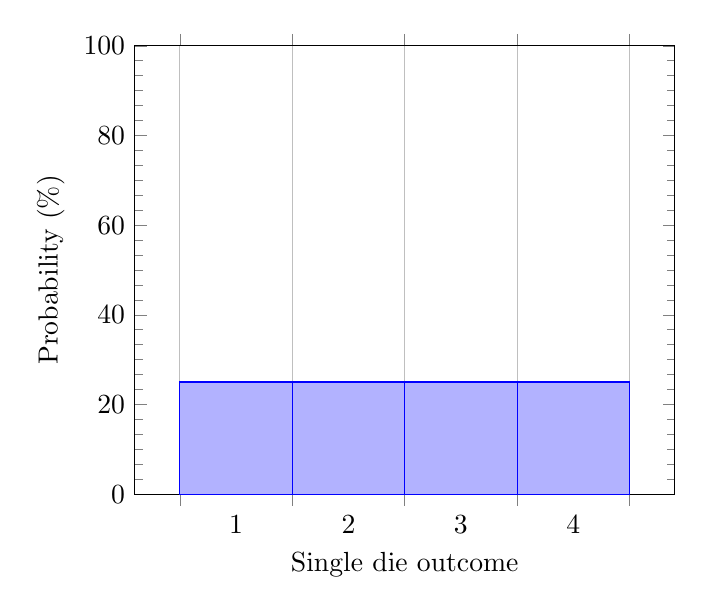
\begin{tikzpicture}
              \begin{axis}[ybar interval, ymax=100,ymin=0, minor y tick num = 5, ylabel=Probability ($\%$), xlabel=Single die outcome]
                \addplot coordinates { (1, 25) (2, 25) (3, 25) (4, 25) (5, 0) };
              \end{axis}
            \end{tikzpicture}
          \end{center}
          \begin{verbatim}
            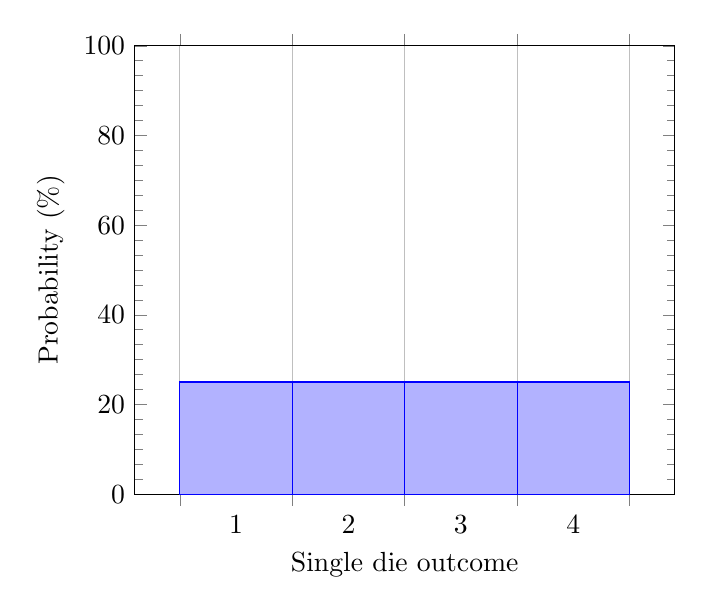
\begin{tikzpicture}
              \begin{axis}[
                ybar interval, 
                ymax=100,ymin=0, 
                minor y tick num = 5, 
                ylabel=Probability ($\%$), 
                xlabel=Single die outcome
                ]
                \addplot coordinates { (1, 25) (2, 25) (3, 25) (4, 25) (5, 0) };
              \end{axis}
            \end{tikzpicture}
          \end{verbatim}
    \item For two four sided dice the table of outcomes looks like\\
          \begin{center}
            \begin{tabular}{c | c c c c}
              $+$ & 1 & 2 & 3 & 4 \\
              \cline{1-5}
              1   & 2 & 3 & 4 & 5 \\
              2   & 3 & 4 & 5 & 6 \\
              3   & 4 & 5 & 6 & 7 \\
              4   & 5 & 6 & 7 & 8 \\
            \end{tabular}
          \end{center}
          So we have 16 possible outcomes and, because the dice are fair, the probability of getting a number is just the number of times that number appears in the
          table divided by 16. Hence the histogram looks like
          \begin{center}
            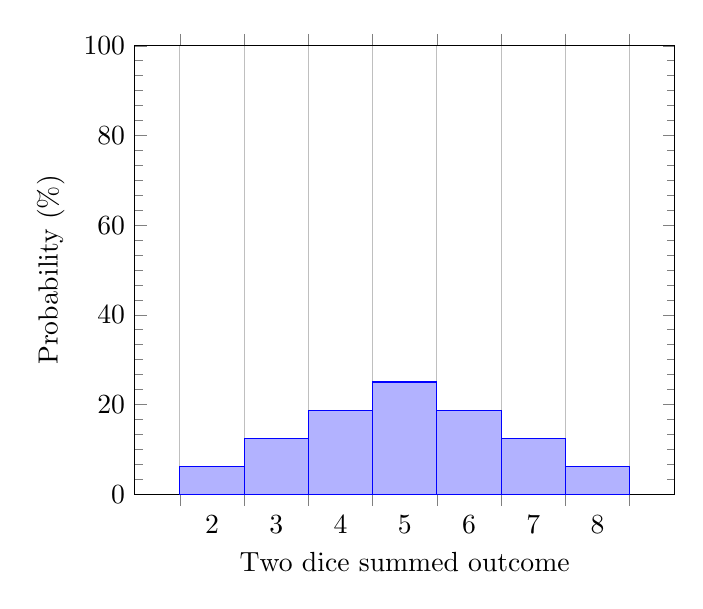
\begin{tikzpicture}
              \begin{axis}[ybar interval, ymax=100,ymin=0, minor y tick num = 5, ylabel=Probability ($\%$), xlabel=Two dice summed outcome]
                \addplot coordinates { (2, 100/16) (3, 200/16) (4, 300/16) (5, 400/16) (6, 300/16) (7, 200/16) (8, 100/16) (9, 0) };
              \end{axis}
            \end{tikzpicture}
          \end{center}
    \item Here we can just take the table from part (b) and ``offset'' it for each outcome of the third die (since the dice are fair, the order doesn't matter).
          This could be represented as a cube of numbers in similar fashion to the previous table but that would be a bit tough to read so I'll show the individual
          third die cases:
          \begin{center}
            \begin{tabular}{c | c c c c}
              Third die rolls 1, $+$ & 1 & 2 & 3 & 4 \\
              \cline{1-5}
              1                      & 3 & 4 & 5 & 6 \\
              2                      & 4 & 5 & 6 & 7 \\
              3                      & 5 & 6 & 7 & 8 \\
              4                      & 6 & 7 & 8 & 9 \\
            \end{tabular},
            \begin{tabular}{c | c c c c}
              Third die rolls 2, $+$ & 1 & 2 & 3 & 4  \\
              \cline{1-5}
              1                      & 4 & 5 & 6 & 7  \\
              2                      & 5 & 6 & 7 & 8  \\
              3                      & 6 & 7 & 8 & 9  \\
              4                      & 7 & 8 & 9 & 10 \\
            \end{tabular},
            \begin{tabular}{c | c c c c}
              Third die rolls 3, $+$ & 1 & 2 & 3  & 4  \\
              \cline{1-5}
              1                      & 5 & 6 & 7  & 8  \\
              2                      & 6 & 7 & 8  & 9  \\
              3                      & 7 & 8 & 9  & 10 \\
              4                      & 8 & 9 & 10 & 11 \\
            \end{tabular}
            \begin{tabular}{c | c c c c}
              Third die rolls 4, $+$ & 1 & 2  & 3  & 4  \\
              \cline{1-5}
              1                      & 6 & 7  & 8  & 9  \\
              2                      & 7 & 8  & 9  & 10 \\
              3                      & 8 & 9  & 10 & 11 \\
              4                      & 9 & 10 & 11 & 12 \\
            \end{tabular}
          \end{center}
          So we end up with 64 possible outcomes and can again express the probability of a given number as the number of times that number appears divided by 64.
          Noting that the probabilites are symmetric about the most common values (because either extreme is the same case in a way, the only way to make 
          the lowest outcome is by all dice rolling their lowest number, and the only way to make the highest is by all dice rolling their highest number) means
          we can just mirror the plot about those most common values which saves a bit of counting. This yields the following histogram,
          \begin{center}
            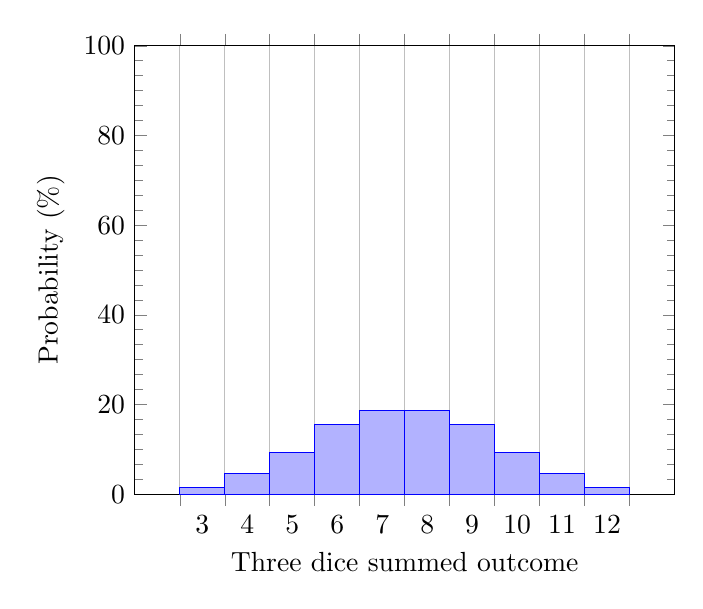
\begin{tikzpicture}
              \begin{axis}[ybar interval, ymax=100,ymin=0, minor y tick num = 5, ylabel=Probability ($\%$), xlabel=Three dice summed outcome]
                \addplot coordinates { (3, 100/64) (4, 300/64) (5, 600/64) (6, 1000/64) (7, 1200/64) (8, 1200/64)
                    (9, 1000/64) (10, 600/64) (11, 300/64) (12, 100/64)
                    (13, 0) };
              \end{axis}
            \end{tikzpicture}
          \end{center}
  \end{enumerate}
\end{soln}
\end{document}